\chapter{Getting started}

The \vcsn \textsc{Project}  has a web site:
\begin{center}
	\code{http://www.vaucanson-project.org}
\end{center}
where all information and documentation on the different components 
of the project, including the present manual, can easily be found and 
downloaded.

\section{Getting \vcsnv}

Naturally, the version \VcsnVersion\xspace of the \vcsn platform can be downloaded
from the \vcsn \textsc{Project} site.

% The version \VcsnVersion\xspace of the \vcsn platform can be downloaded
% from 
\medskip 
Alternatively, it can also be found at\\
\PushLine
\code{http://vaucanson.lrde.epita.fr/Vaucanson\VcsnVersion}.
\PushLine

Other previous versions of the \vcsn platform can be downloaded
from \\
\PushLine
\code{http://vaucanson.lrde.epita.fr/}.
\PushLine
% Please note this manual is not meant to be backward compatible with
% \vcsn versions prior to \VcsnVersion.

\Cave
This version \VcsnVersion\xspace is not fully backward compatible 
with earlier versions and 
this manual is not meant to document the differences with
\vcsn versions prior to \VcsnVersion\xspace (which had never been really 
documented).
In one word, no other version than \vcsnv or \vcsn\VcsnVrsnOld\xspace should be used.



\section{Licensing}
\vcsnv is a free software released under the GNU General
Public Licence version 2. 
More information on this license is to be found at
\code{http://www.gnu.org/licenses/gpl-2.0.txt} (a copy of
this license is included in each copy of \vcsn in the file
\emph{COPYING}).

Beware that the license for the next versions of \vcsn will
probably be different (although \vcsn will stay an open and free
software).

\section{Prerequisites}
\label{sec:pre-req}%

\begin{description}
\item[\Cpp compiler] \code{G++ 4.x} or later.

\item[\XML] The \XML I/O system is based on the use of the Apache \code{Xerces}
  \Cpp library version 2.7 or later (\code{http://apache.org/xerces-c/}). (On
  Ubuntu/Debian, install packages with names similar to: \code{libxerces28} and \code{libxerces28-dev},
  or \code{libxerces-c3.1} and \code{libxerces-c-dev}),
\Indextt{Xerces}%

\item[\code{Boost}] \code{Boost} provides free peer-reviewed
portable \Cpp source
  libraries (On Ubuntu/Debian, install the following packages:
  l\code{ibboost-dev}, \code{libboost-serialization-dev}, \code{libboost-graph},
  \code{libboost-graph-dev}).
  \vcsn is compatible with \code{Boost} versions \code{1.34} or later.
\Indextt{Boost}%

\item[\code{Ncurses}] needed for building \tafkit  (On Ubuntu/Debian, install
  the following packages: \code{libncurses5}, \code{libncurses-dev}).
\Indextt{Ncurses}%

\item[\code{Graphviz}] The display of automata is made using AT\&T \code{GraphViz}
  application (On Ubuntu/Debian, install the following package: \code{graphviz}).
\Indextt{Graphviz}%

\end{description}

\section{Building \vcsn}
\label{sec:bui-ld}%


Detailed information is provided in both \code{INSTALL} and \code{doc/README.txt}
files. The following installation commands will install \vcsn in
'\code{/usr/local}'.

\begin{shell}
$ cd vaucanson-\VcsnVersion
$ ./configure
$ make
$ sudo make install
\end{shell}%


Depending on the architecture, both \code{Boost} and \code{Xerces} might be located
in non-standard directories. 
The location of these
libraries may known via the following command:

\begin{shell}
$ whereis boost
\end{shell}%

This command returns the paths to \code{Boost} headers. 
These directories are then
specified  to the \code{configure} file by means of
two environment variables: \code{CPPFLAGS} for the header files and \code{LDFLAGS}
for the library files. 
For instance, if \code{Boost} headers are located
in:\\
'\code{/usr/user\_name/home/my\_path\_to\_boost/include}' and its library
files in:\\
'\code{/usr/user\_name/home/my\_path\_to\_boost/lib}', the
following configure line should be invoked:

\begin{shell}
$ ./configure   CPPFLAGS='-I/usr/user\_name/home/my\_path\_to\_boost/include'
                LDFLAGS='/usr/user\_name/home/my\_path\_to\_boost/lib'
\end{shell}%

If \vcsn is not installed but only compiled,
the \tafkit binaries are to be found in the directory
'\code{vaucanson-\VcsnVersion/taf-kit/tests/}' (This directory
contains wrappers
around the real \tafkit programs from '\code{vaucanson-\VcsnVersion/taf-kit/src/}'
that enable them to run locally).

\section{Mac\xmd OS\xmd X specifics}

The installation process of \vcsn
and its dependencies on Mac\xmd OS\xmd X may be less straightforward
than onto other Linux systems.

% First, the Mac\xmd OS\xmd X system should be up-to-date before
% going through the rest of the installation process.

First, the \code{macports} software will be used to get all the
prerequisites and should be installed first on the computer
(see \code{http://www.macports.org/}).
A complete guide
to its installation is available from \code{http://guide.macports.org/}.
If \code{macports} is already installed, it should be made up-to date
by synchronising the local port tree with the global \code{macports}
ports by the following command.
\begin{shell}
$ sudo port selfupdate
\end{shell}%

Three libraries are to be installed in order to
build \vcsn (see Prerequisite for details):
\code{Boost},
\code{Xerces}, and
\code{Ncurses}.
\begin{shell}
$ sudo port install ncurses
...
$ sudo port install boost
...
$ sudo port install xercesc
...
$
\end{shell}%
Note that executing each of these commands may take a while
(especially when installing \code{Boost}).
%
By default, \code{macports} will install each of these three
libraries in the \code{/opt/local} directory, which is not standard
with respect to the Unix organisation.
In order to build \vcsn, this directory is therefore to be specified
to the \code{configure} command by the following options:
\begin{shell}
$ ./configure CPPFLAGS='-I/opt/local/include' LDFLAGS='-L/opt/local/lib'
\end{shell}%

Moreover, if the installed version of \code{Boost}  is greater than
or equal to~1.44 it is necessary to add another option to the
\code{configure} command:
\begin{shell}
$ ./configure CPPFLAGS='-I/opt/local/include -DBOOST\_SPIRIT\_USE\_OLD\_NAMESPACE'
              LDFLAGS='-L/opt/local/lib'
\end{shell}%
The installation is then to be completed by the usual two commands:
\begin{shell}
$ make
$ sudo make install
\end{shell}%

\section{Improving the display quality}

As long as a dedicated graphical interface is not fully operational, 
displaying automata is processed by the \code{Graphviz} application, which 
is normally launched
in an \code{X11} window.
It is to be acknowledged that the call to \code{Graphviz} by \tafkit
is not well-tuned and that the output is rather poor.
It is not too difficult however to get a rendering of
automata of much better quality (\cf \figur{gra-viz}).
This can be done in three steps and in a slightly different way for 
Mac and Linux users.

\subsection{\code{Graphviz} for Mac}

First download the \code{Graphviz} application for Mac from
\code{www.pixelglow.com/graphviz/}.
Although already old and outdated by the \code{2.xx} versions, the
\code{1.13 (v16)} version is recommended as the settings is easier to
handle in that version.
Complete the installation by putting the \code{Graphviz.app} folder
in the \code{Applications} folder.

Second, write the following script in a file called \code{dotty}:
\begin{shell}
#! /bin/sh
if [ "x$1" = x- ]; then
 cat >/tmp/tmpdotty$$.dot
 open -W -a Graphviz /tmp/tmpdotty$$.dot
 rm -f /tmp/tmpdotty$$.dot
else
 open -W -a Graphviz "$1"
fi
\end{shell}%

Finally, make this file executable, store it in a folder, and put the
full name of this folder in the \code{PATH} variable before
\code{/usr/local/bin:} and \code{/usr/X11/bin:}.
The appearance of the automata will be determined by fixing the
settings in the interface.


\subsection{\code{Graphviz} for Linux}

For Linux users, the process is almost same except that the program 
required is \code{xpdf} and the \code{dotty} script is:

\begin{shell}
#!/bin/sh
f=/tmp/pd$$.png
if test "x$1" = x-; then
  dot -Tpdf > $f
else
  dot -Tpdf "$@" > $f
fi
xpdf $f
rm -f $f
\end{shell}%


\begin{figure}[ht]
    \centering
\includegraphics[scale=0.25]{figures/a1-dotty.ps}
\ee
\includegraphics[scale=0.5]{figures/a1-gv.ps}
\caption{Two versions of the \code{Graphviz} application}
\label{fig:gra-viz}%
\end{figure}


\section{VGI}

The availability of the Graphical User Interface \vgi, developped at 
NTU, is one of the novelty of \vcsnv with respect to \vcsnvo.
Every instance of \tafkit has a function \code{gui} that launches 
\vgi (\cf \secti{taf-io-fun}).
For this function to work, \tafkit needs to be specified where is \vgi.

Download the \code{vgi.jar} archive from 
\code{http://vaucanson-project.org/resources/vgi.jar},  store it in a 
folder denoted by \code{/path/to/vgi/folder}  in the following.

There is two methods to specify to \vcsn where this archive is 
stored: either by setting the environment variable \code{VGIJAR}
with the command:

\begin{shell}
$ export VGIJAR=/path/to/vgi/folder/vgi.jar
\end{shell}

\noindent
or by puting the following script named "\code{vgi}" in a directory of the 
path (for instance \code{/usr/local/bin}): 

\begin{shell}
#!/bin/sh
exec java -jar /path/to/vgi/folder/vgi.jar "$@"
\end{shell}

\noindent
and making it executable. 
A call to the \code{gui} function will then open a window such as the 
one shown at \figur{vgi} (\cf \apndx{vgi}).


\begin{figure}[ht]
    \centering
\includegraphics[width=3in]{\VGIFig fig14.eps}
\caption{The \vgi window }
\label{fig:vgi}%
\end{figure}

%%%%%%%%%%%
\endinput
